\chapter{Theoretische Grundlagen}
\label{chap:theoretische_grundlagen} Dieses Kapitel führt in die theoretischen Grundlagen
ein, die in dieser Arbeit benötigt werden. Den ersten Teil bilden die domänenspezifischen
Grundlagen \ref{sec:domänenspezifisch}, welche genauer darauf eingehen, welchen Inhalt
die zu bearbeitenden Bilder bieten und wie dieser zu verstehen ist. Abschnitt
\ref{sec:technologisch} geht hierbei auf verschiedenen Technologien ein, die eine
wichtige Rolle spielen. Der Abschnitt \ref{sec:verwwandte_arbeit} geht auf die
Arbeit vin \citet{hoffmann2020} ein und legte damit den Grundstein diese vorliegenden
Arbeit. Die Abschnitte \ref{sec:3d_slicer} und \ref{sec:architektonisch} führen
in Softwareentwicklungsthemen ein, die zum erstellen einer \textit{3D Slicer
Extention} wichtig sind.

\section{Domänenspezifisch}
\label{sec:domänenspezifisch} Wie bereits aus dem Kapitel \ref{chap:einleitung}
Einleitung klar wurde, handelt es sich bei den Micro-CT Bilder um Zahnbilder,
die aufgrund einer Karieserkrankung entfernt wurden. Um zu verstehen, wie eine
CT-Aufnahme eines Zahns augeteilt werden soll, ist es hilfreich zu verstehen,
wie ein Zahn aufgebaut ist.

\begin{minipage}{0.40\textwidth}
	Die Abbildung \ref{fig:aufbau_eines_zahnes} zeigt den groben Aufbau eines Zahnes
	nach \citet[Seite 17]{lehmann2012Zahnheilkunde}. Zu sehen ist, dass das Denit oder
	auch Zahnbein genannt, den Großteil eines Zahnes einnimmt. Im bereich der Zahnkrone
	wird das Dentin von Zahnschmelz überzogen. Der Zahnschmelz ragt in die
	Mundhöle und ist nach \cite[Seite 41]{lehmann2012Zahnheilkunde} das härteste
	Material im menschlichen Körper. In der Mitte des Zahnes befindet sich Weichgewebe,
	welches als Pulpa bezeichnet wird vgl. \citep[Seite ]{lehmann2012Zahnheilkunde}.
\end{minipage}
\hfill
\begin{minipage}{0.50\textwidth}
	\centering
	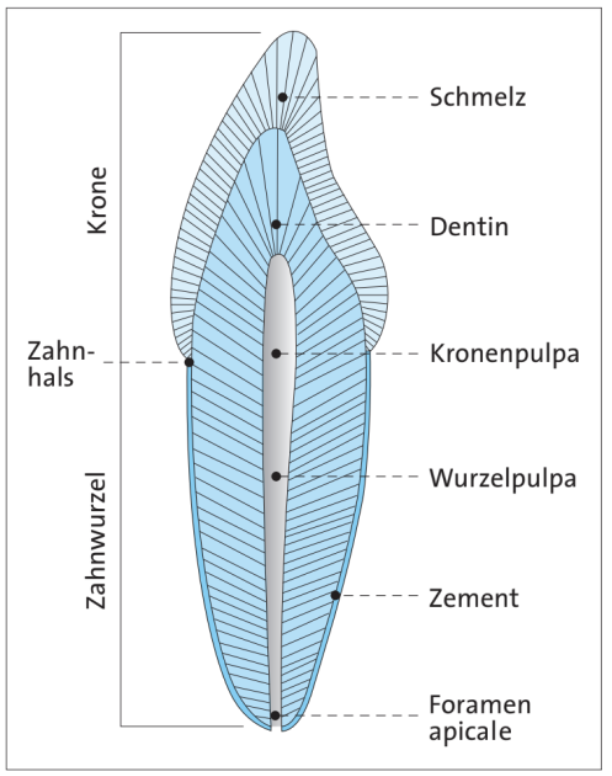
\includegraphics[scale=0.50]{img/aufbau_eines_zahns.jpg}
	\captionof{figure}{Aufbau eines Zahnes nach \citet{lehmann2012Zahnheilkunde}} \label{fig:aufbau_eines_zahnes}
\end{minipage}

Für die Bearbeitung von Micro-CT Aufnahmen sind die Bereich Schmelz Dentin und Pulpa
von besonderer Bedeutung. Betrachtet man eine CT wie es zu begin in der
Abbildung \ref{fig:ct_aufnahme_eines_zahns} gezeigt wurde, so bilden diese 3 Gewebearten
die unterschiedlichen Grauwerte in einem CT-Bild. \\ \textbf{Pulpa:} Die Pulpa unterscheidet
sich hierbei nur wenig vom Hintergrund, da sie als einzige der drei Hauptteile
eines Zahnes eine Weichgewebe ist und bei einer Röntgenaufnahme nicht absorbiert.
Geht man weiter von innen nach außen, so ist der nächste Zahnteil auf einem CT
das Zahnbein. \\ \textbf{Dentin:} Das Dentin ist laut \citet[Seite 41]{lehmann2012Zahnheilkunde}
eine Hartsubstanz, die dem Kieferknochen sehr nahe steht. So kommt es, dass dieser
Teil schon deutlich besser auf einem CT zu erkennen ist. Den äußersten Teil in
der Mundhöle bildet das Zahnschmelz. \\ \textbf{Schmelz:} Der Schmelz ist wie
bereits erwähnt, der härteste Teil im menschlichen Körper und aus diesem Grund auch
am hellsten auf dem CT zu erkennen. Die folgenden Abbildung
\ref{fig:pulpa_dentin_schmelz} sollen durch gegenüberstellung den Zusammenhang
zwischen einem CT-Bild und einer Zahnzeichnung verdeutlichen.

\begin{figure}[h]
	\centering
	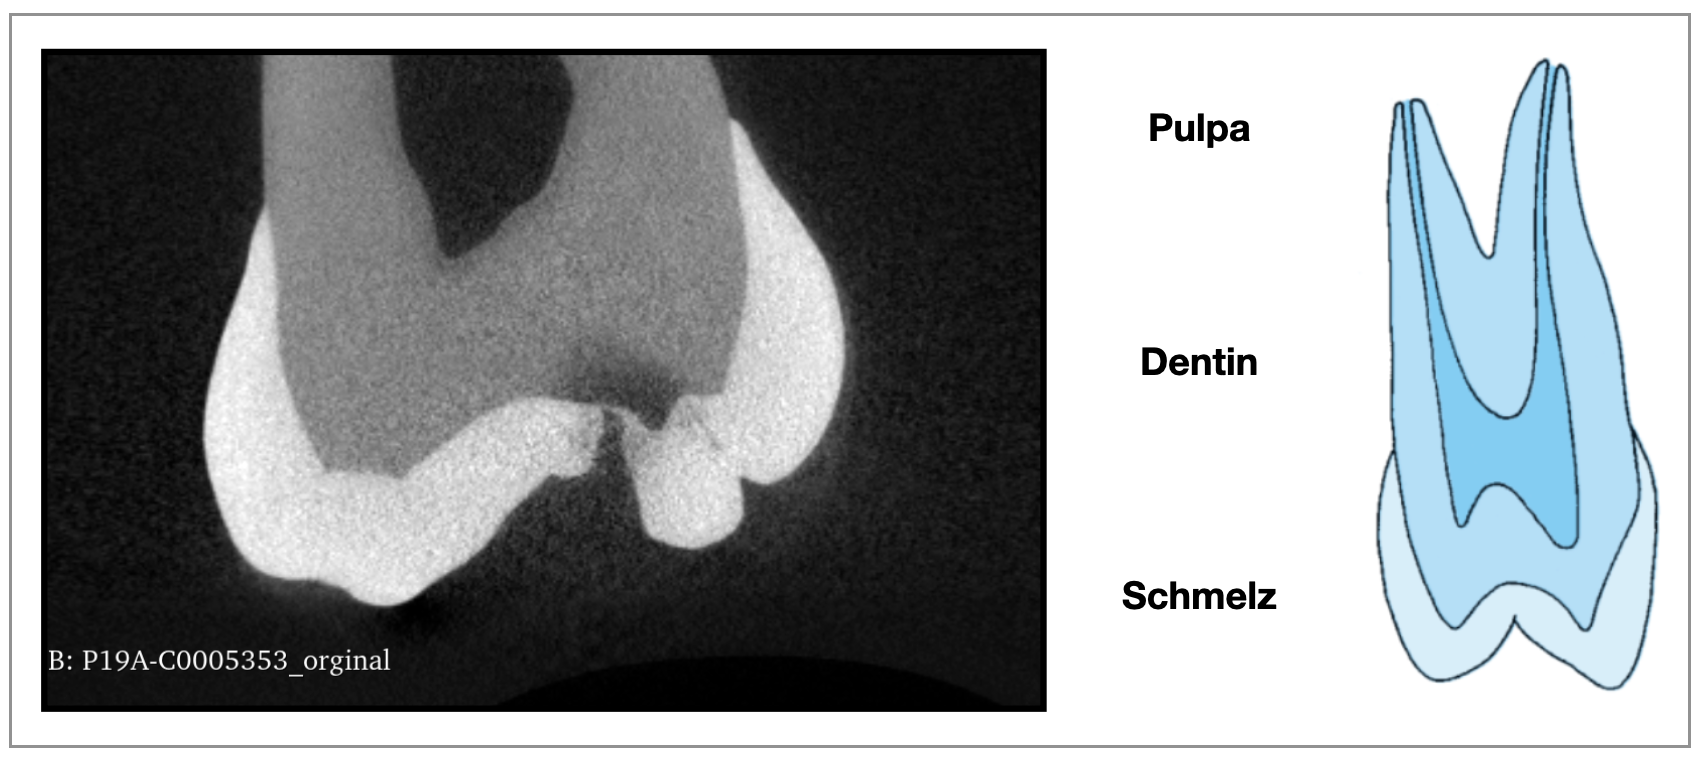
\includegraphics[width=0.9\textwidth]{
		img/Bildschirmfoto 2024-11-22 um 15.13.24.jpg
	}
	\caption{Darstellung von Pulpa, Dentin und Schmelz auf einer CT-Aufnahme (link)
	und einer Zeichnung (rechts) nach \citet[Seite 29]{lehmann2012Zahnheilkunde}. }
	\label{fig:pulpa_dentin_schmelz}
\end{figure}

Mit diesem Domänenwissen kann ein Schritt weiter gegangen werden, sodass der
Fokus nun auf die CT-Bilder gesetzt wird. Das Kapitel \ref{sec:technologisch} Technologien
führt die Technologie der Computertomografie tiefer ein. Mit diesem
Domänenwissen kann ein Schritt weiter gegangen werden, sodass der Fokus nun auf die
CT-Bilder gesetzt wird. Das Kapitel \ref{sec:technologisch} Technologien führt
die Technologie der Computertomografie tiefer ein.£

\section{Technologisch}
\label{sec:technologisch} Dieser Abschnitt erläutert federführend die Technologie
der Micro-CT bilder und und deren weitere Bearbeitung. Hierbe soll mit der
Computertomografie selbst begonnen werden. Für die Einführung in die Bearbeitung
der Micro-CT Bilder bietet das Pipelinmodell von \citet[Seite 50]{handels2000} eine
gut Richitline. Er beschreibt mit dieser Visualisierungs-Pipeline Schritte, die bei
der Bearbeitung und dreidimensonalen Darstellung von CT-Aufnahmen notwendig sind
vgl. \citep[Seite 50]{handels2000}.

\subsection{Computertomografie}
\label{subsec:computertomografie} Die Efindung der Computertomografie (CT) war
ein Quantensprung in der Geschichte der Medizin. Sie ist aus heutigen Diagnosen nicht
mehr wegzudenken. Ein Micro-CT Bild ist laut \citet[Abstract]{baird2017} ein
Menge hochauflösender Bilder, die wie ein Stapel zusammengelegt werden. Der
Aspekt Micro deutet dabei darauf hin, dass es eine miniaturisierte Ausführung eines
üblichen Kegelstrahl-CTs ist so \citet[Seite 340]{buzug2011}. Eine andere
Definition erläutert \citet{lehmann2013bildverarbeitung}. Er beschreibt die
Computertomografie als Projektionen einzelner Ebenen im Untersuchungsobjekt. Die
Technologie, mit der diese Bilderstapel aufgenommen werden ist unter der
Röntgentechnik oder auch X-Ray bekannt. Die Röntgenstrahlung ist eine Form der elektromagnetischen
Strahlung, ähnlich wie da sichtbare Licht so das \citet{nib2024}. Anders als das
Licht, haben die Röntgenstrahlen eine viel höhere Energie. Das führt dazu, dass man
mit dieser elektromagnetischen Strahlung viele Objekte durchdringen kann. So
auch Gewebeteile eines Zahnes vgl. \citep{nib2024}. Die Abbildung \ref{fig:spectrum}
zeigt diese elektromagnetische Spektrum.

\begin{figure}[h]
	\centering
	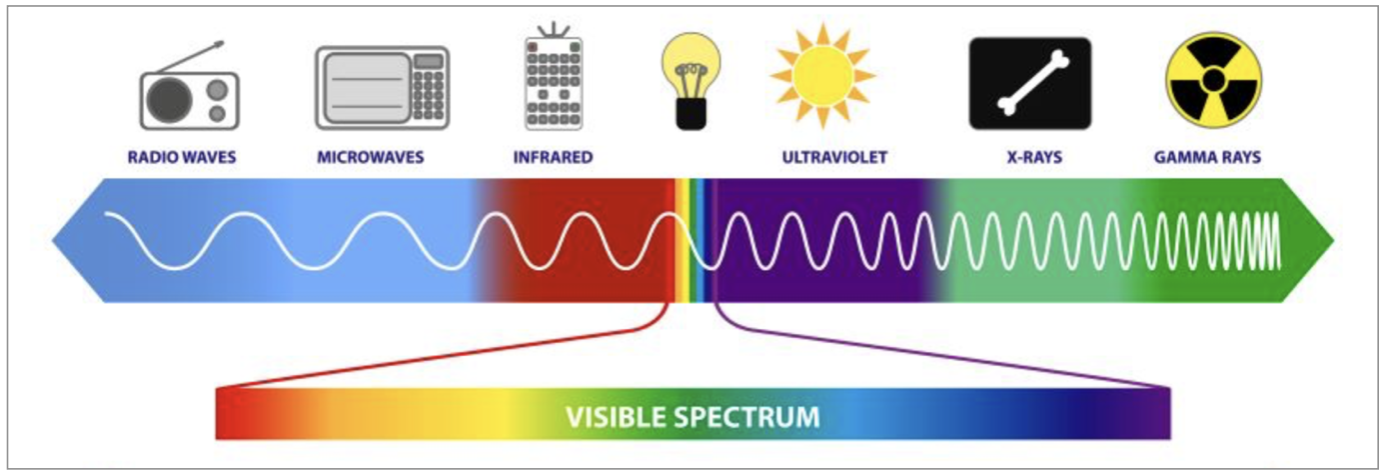
\includegraphics[width=0.9\textwidth]{img/spectrum.jpg}
	\caption{Einordnung der Röntgenstrahlung nach dem \citet{nib2024}}
	\label{fig:spectrum}
\end{figure}

Durchdringt ein solcher Röntgenstrahl ein Untersuchungsobjekt, werden die Details
auf Grund der Wechselwirkung mit Materie auf einer CT-Probe sichtbar. Die
bekannteste Wechselwirkung ist die Absorbtion. Mit der steigerung der Atomzahl in
einem Element nimmt auch die Absorbtion eines Materials zu, sodass es leicht ist
verschiedenen Materialien in einer CT-Aufnahme zu unterscheiden \citep{nib2024}.

Für eine Micro-CT Aufnahme bedarf es spezieller Technik. Es gibt unterschiedliche Firmen,
welche die unterschiedlichsten Modelle anbieten. Im Falle der Zahnklinik an der LMU in
München Handelt es sich um ein Micro-CT 40 der Firma \citet{scanco2024}. Diese Gerät erstelt
Aufnahmen mittels Röntgenstrahlung und erstehlt daraus mit Hilfer der Computertomografie ein
dreidimensonales Bild, welches im Format \textit{.isq} abgelegt wird. Wie das Nächste Kapitel
beschreiben wird ist der Speicherumfang den solch ein Bild benötigt, deutlich zu groß. Es bedarf
einer technik, mit der die Aufnahmen auf eine handhabbare Größe schrumpfen.


\subsection{Datensätze}

\subsection{Filter}

\subsection{Segmentierung}

\section{Verwandte Arbeit}
\label{sec:verwwandte_arbeit}

\section{3D Slicer}
\label{sec:3d_slicer}

\subsection{Extention Manager}

\subsection{Python Umgenbung}

\subsection{MRML Datenstruktur}

\subsection{Qt-Designer}

\section{Architektonisch}
\label{sec:architektonisch}